\documentclass[tikz,border=0pt]{standalone}
\usepackage[utf8]{inputenc}
\usepackage{xcolor}

% Card dimensions - playing card ratio
\newcommand{\cardwidth}{250pt}
\newcommand{\cardheight}{350pt}

% KidLisp syntax colors (from kidlisp.mjs)
\definecolor{cardbg}{HTML}{FFF9C0}
\definecolor{codebg}{HTML}{1A1612}
\definecolor{titlecolor}{HTML}{2D2A24}
\definecolor{bodycolor}{HTML}{4A4540}
\definecolor{categorycolor}{HTML}{888888}

% KidLisp syntax highlighting colors
\definecolor{klparen}{HTML}{888888}      % Gray for parentheses
\definecolor{klfunction}{HTML}{FF6B6B}   % Coral/red for functions like 'line', 'box'
\definecolor{klnumber}{HTML}{4ECDC4}     % Cyan for numbers
\definecolor{klstring}{HTML}{FFE66D}     % Yellow for strings
\definecolor{klvar}{HTML}{95E1D3}        % Mint for variables like 'width', 'height'

% Diagram colors
\definecolor{gridcolor}{HTML}{DDDDDD}
\definecolor{linecolor}{HTML}{FF6B6B}

\begin{document}
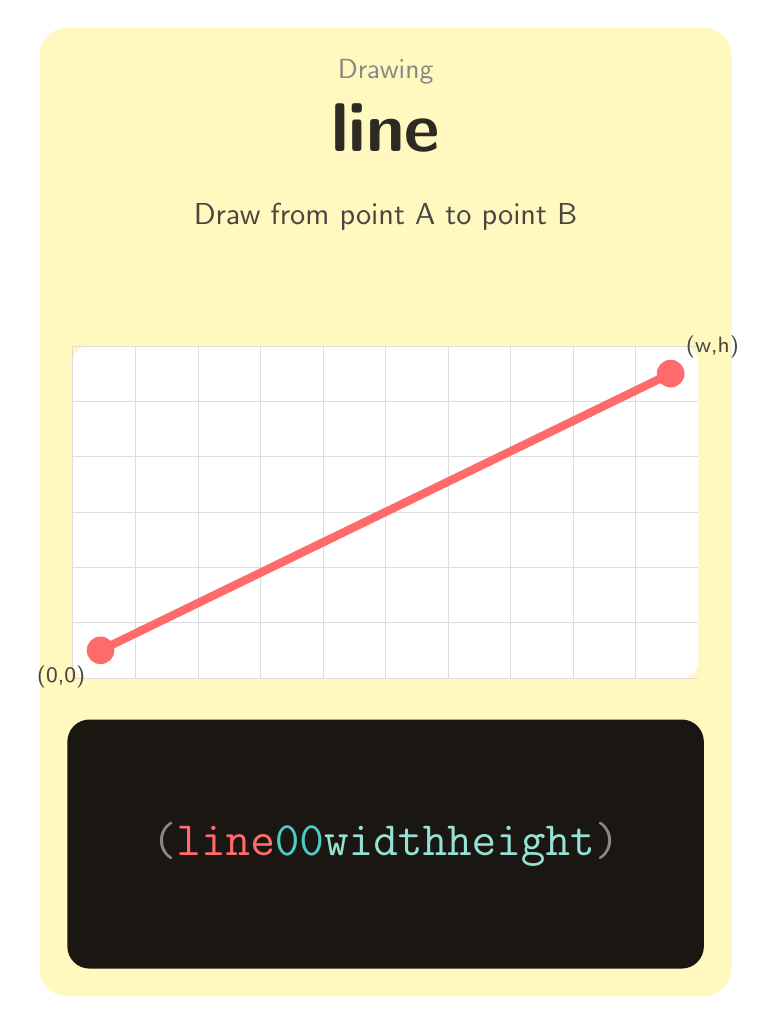
\begin{tikzpicture}
  % Card background
  \fill[cardbg, rounded corners=10pt] (0,0) rectangle (\cardwidth, \cardheight);
  
  % Category at top
  \node[anchor=north, font=\sffamily\fontsize{10}{12}\selectfont\color{categorycolor}] 
    at (0.5*\cardwidth, \cardheight-8pt) {Drawing};
  
  % Title - big and bold
  \node[anchor=north, font=\sffamily\bfseries\fontsize{28}{32}\selectfont\color{titlecolor}] 
    at (0.5*\cardwidth, \cardheight-24pt) {line};
  
  % Description - concise
  \node[anchor=north, text width=\cardwidth-24pt, font=\sffamily\fontsize{11}{14}\selectfont\color{bodycolor}, align=center] 
    at (0.5*\cardwidth, \cardheight-60pt) {Draw from point A to point B};
  
  % === VISUAL DIAGRAM ===
  % Grid background
  \begin{scope}[shift={(12pt, 115pt)}]
    \def\diagramwidth{226pt}
    \def\diagramheight{120pt}
    
    % Grid background
    \fill[white, rounded corners=6pt] (0,0) rectangle (\diagramwidth, \diagramheight);
    
    % Grid lines
    \foreach \x in {0,22.6,...,226} {
      \draw[gridcolor, line width=0.3pt] (\x pt, 0) -- (\x pt, \diagramheight);
    }
    \foreach \y in {0,20,...,120} {
      \draw[gridcolor, line width=0.3pt] (0, \y pt) -- (\diagramwidth, \y pt);
    }
    
    % The line itself (diagonal from corner to corner)
    \draw[linecolor, line width=3pt, line cap=round] (10pt, 10pt) -- (216pt, 110pt);
    
    % Start point marker
    \fill[linecolor] (10pt, 10pt) circle (5pt);
    \node[anchor=north east, font=\sffamily\fontsize{8}{10}\selectfont\color{bodycolor}] 
      at (8pt, 8pt) {(0,0)};
    
    % End point marker  
    \fill[linecolor] (216pt, 110pt) circle (5pt);
    \node[anchor=south west, font=\sffamily\fontsize{8}{10}\selectfont\color{bodycolor}] 
      at (218pt, 112pt) {(w,h)};
  \end{scope}
  
  % === CODE BLOCK ===
  \fill[codebg, rounded corners=8pt] (10pt, 10pt) rectangle (\cardwidth-10pt, 100pt);
  
  % Code with syntax highlighting - positioned for single line
  \node[anchor=center] at (0.5*\cardwidth, 55pt) {
    {\fontsize{16}{20}\selectfont\ttfamily
      \textcolor{klparen}{(}%
      \textcolor{klfunction}{line}%
      \textcolor{white}{ }%
      \textcolor{klnumber}{0}%
      \textcolor{white}{ }%
      \textcolor{klnumber}{0}%
      \textcolor{white}{ }%
      \textcolor{klvar}{width}%
      \textcolor{white}{ }%
      \textcolor{klvar}{height}%
      \textcolor{klparen}{)}%
    }
  };
\end{tikzpicture}
\end{document}
